\documentclass[11pt,compress,t,notes=noshow, aspectratio=169, xcolor=table]{beamer}

\usepackage{../../style/lmu-lecture}
% Defines macros and environments
\usepackage{bbm}
% basic latex stuff
\newcommand{\pkg}[1]{{\fontseries{b}\selectfont #1}} %fontstyle for R packages
\newcommand{\lz}{\vspace{0.5cm}} %vertical space
\newcommand{\dlz}{\vspace{1cm}} %double vertical space
\newcommand{\oneliner}[1] % Oneliner for important statements
{\begin{block}{}\begin{center}\begin{Large}#1\end{Large}\end{center}\end{block}}


%new environments
\newenvironment{vbframe}  %frame with breaks and verbatim
{
 \begin{frame}[containsverbatim,allowframebreaks]
}
{
\end{frame}
}

\newenvironment{vframe}  %frame with verbatim without breaks (to avoid numbering one slided frames)
{
 \begin{frame}[containsverbatim]
}
{
\end{frame}
}

\newenvironment{blocki}[1]   % itemize block
{
 \begin{block}{#1}\begin{itemize}
}
{
\end{itemize}\end{block}
}

\newenvironment{fragileframe}[2]{  %fragile frame with framebreaks
\begin{frame}[allowframebreaks, fragile, environment = fragileframe]
\frametitle{#1}
#2}
{\end{frame}}


\newcommand{\myframe}[2]{  %short for frame with framebreaks
\begin{frame}[allowframebreaks]
\frametitle{#1}
#2
\end{frame}}

\newcommand{\remark}[1]{
  \textbf{Remark:} #1
}


\newenvironment{deleteframe}
{
\begingroup
\usebackgroundtemplate{\includegraphics[width=\paperwidth,height=\paperheight]{../style/color/red.png}}
 \begin{frame}
}
{
\end{frame}
\endgroup
}
\newenvironment{simplifyframe}
{
\begingroup
\usebackgroundtemplate{\includegraphics[width=\paperwidth,height=\paperheight]{../style/color/yellow.png}}
 \begin{frame}
}
{
\end{frame}
\endgroup
}\newenvironment{draftframe}
{
\begingroup
\usebackgroundtemplate{\includegraphics[width=\paperwidth,height=\paperheight]{../style/color/green.jpg}}
 \begin{frame}
}
{
\end{frame}
\endgroup
}
% https://tex.stackexchange.com/a/261480: textcolor that works in mathmode
\makeatletter
\renewcommand*{\@textcolor}[3]{%
  \protect\leavevmode
  \begingroup
    \color#1{#2}#3%
  \endgroup
}
\makeatother


\providecommand{\tightlist}{%
  \setlength{\itemsep}{0pt}\setlength{\parskip}{0pt}}

%\setbeamerfont{footnote}{size=\tiny}
\usepackage[hang,flushmargin]{footmisc}
\renewcommand*{\footnotelayout}{\tiny}
\renewcommand*{\thefootnote}{} %\fnsymbol{footnote}

% https://tex.stackexchange.com/questions/30720/footnote-without-a-marker
% \makeatletter
% \def\blfootnote{\gdef\@thefnmark{}\@footnotetext}
% \makeatother

% https://tex.stackexchange.com/questions/357717/beamer-allowframebreaks-option-and-vertical-spacing-when-using-lists-itemize
% \setbeamertemplate{frametitle continuation}{%
%     (\insertcontinuationcount)%
%     \ifnum\insertcontinuationcount>1%
%     \vspace*{\topsep}%
%     \else%
%     %
%     \fi%
% }

\newcommand{\open}{}
\newcommand{\close}{}

\title{Interpretable Machine Learning}
% \author{LMU}
%\institute{\href{https://compstat-lmu.github.io/lecture_iml/}{compstat-lmu.github.io/lecture\_iml}}
\date{}

\begin{document}

%Gliederung:
%- Intro with examples, motivation, problems
%- standard fANOVA calculation + example
%- from that intuition & motivation: h-statistic
%- conditions + theory
%- other methods (gen fANOVA, ALE)

% \newcommand{\titlefigure}{figure/open_blackbox}
\newcommand{\titlefigure}{figure/25-05-31_Hooker_2004_graph_fANOVA}
\newcommand{\learninggoals}{
\item Basic idea of additive functional decompositions
\item Motivation and usefulness of functional decompositions
\item Difficulty of obtaining or even defining a functional decomposition}

\lecturechapter{Introduction to Functional Decomposition}
\lecture{Interpretable Machine Learning}


\begin{frame}{Recap: interaction}
    Recap: Interactions between features: The effect of some features on the prediction output depends on (one or more) other features \\
    This cannot be captured by the main feature effects alone (i.e. by a GAM).
    We want to know, which parts are attributed to effects of single features (s.o. feature effect methods), and which to interactions.

    \textit{
    TO DO: After introducing PDPs and PD-functions more generally in chapter 3, we would want to introduce H-statistic as a measure / as a possible definition for interactions, maybe even in the general case (i.e. the H-statistic for testing for an \(n\)-way interaction between \(n\) many features). \\
    First introduce the more general concept of \(k\)-way interactions between any \(k\) groups of variables. \\
    Remember EBMs at this point: There, strong interactions were defined via reduction in RSS compared to a univariate model / a GAM -> exactly same idea / same formula
    }

\end{frame}

\begin{frame}{First Example: Additive decomposition}

    \begin{example}

    Consider
    $$
    \fh(x_1, x_2) = 4 - 2x_1 + 0.3 e^{x_2} + |x_1|x_2
    $$
    % The function \( \fh(x_1, x_2) = 4 - 2x_1 + 0.3 e^{x_2} + |x_1|x_2 \) depends on two features, and contains the interaction \( |x_1|x_2 \) between the two features.

    \begin{itemize}
        \item Idea: Additive decomposition depending on which features used:
        \begin{equation}\label{eq:func_decomp_first_min_example}
        \begin{aligned}
            & g_0(x_1, x_2) = 4 & \text{ Part depending on no features at all (intercept)}  \\
            &
            \left.\begin{aligned}
                & g_1(x_1, x_2) = 2x_1 \\
                & g_2(x_1, x_2) = 0.3 e^{x_2}
            \end{aligned}\right\}
                & \text{ Parts depending on a single feature (main effects)}  \\
            & g_{1,2}(x_1, x_2) = |x_1|x_2 & \text{ Part depending on both features (interaction)}  \\
        \end{aligned}
        % \begin{matrix}
        %     g_0(x_1, x_2) = 4 &  \text{ Parts depending on no features at all (constant)}  \\
        %     g_1(x_1, x_2) = 2x_1 & \text{ Parts depending on a single feature (main effects)} \\
        %     g_1(x_1, x_2) =  0.3 e^{x_2} & \\
        %     g_{1,2}(x_1, x_2) = |x_1|x_2 & \text{ Part depending on both features (interaction)}  \\
        % \end{matrix}
        \end{equation}
        \item[$\leadsto$] single terms with immediate interpretation, full understanding of the model
        
        \item[$\leftrightarrow$] Not possible with effects of single features (e.g. PDPs) or GAM surrogate model (miss interaction part)
    
        % Using a GAM or looking at the effects of single features will not allow us to fully understand the function. 
        
        % The single terms enable immediate interpretation (effects of single features, single interactions etc). \\
        
    \end{itemize}

    \end{example}

\end{frame}

% \begin{frame}{First Example: Additive decomposition}

    % [visualization] 

    % In general, functional form is unknown, but goal is to find such a decomposition:
    % Given a function / black-box model \(\fh: \R^2 \to \R\), we want to find a decomposition

    % \begin{equation}
    %     \fh(x_1, x_2) =  g_{0} + g_1(x_1) + g_2(x_2) + g_{\open 1, 2 \close}(x_1, x_2)
    % \end{equation}
    
% \end{frame}

\begin{frame}{Another Example: Additive decomposition}

\textbf{Goal} in general:
Given a black-box model \(\fh: \R^2 \to \R\), find a decomposition
\begin{equation}
    \fh(x_1, x_2) =  g_{0} + g_1(x_1) + g_2(x_2) + g_{\open 1, 2 \close}(x_1, x_2)
\end{equation}

\textit{TO DO: Better use a real-world example, only image here necessary for illustration purposes}

\begin{example}
% \textbf{Example:}
$\fh(\xv) = 2 + x_1^2 - x_2^2 + x_1 \cdot x_2$ (e.g., for $x_1 = 5$ and $x_2 = 10$ we get $\fh(\xv) = -23$)

\begin{itemize}
    \item Computation of components using feature values $x_1 = x_2 = (-10, -9, \ldots, 10)^\top$ gives:
        \includegraphics[width = \textwidth]{figure/decomposition}
\end{itemize}
    
\end{example}
\end{frame}

\begin{frame}{Another example}

    \begin{example}

        % Consider the function

        \begin{equation*}
            \fh(x_1, x_2, x_3) = - 2x_1 - 2\sin(x_3) + |x_1|x_2 + 0.5 x_1 x_2 x_3 - \sin(x_2 x_3) + 1
        \end{equation*}

        % We can again find the additive decomposition by reading from the functional formula, but some terms are empty, because certain types of effects and interactions are not present:
        Again, read additive decomposition from formula:
        \begin{equation}\label{eq:func_decomp_second_min_example}
        \begin{aligned}
            & g_0(x_1, x_2, x_3) = 1 & \text{ constant part, no effects}  \\
            &
            \left.\begin{aligned}
                & g_1(x_1, x_2, x_3) = - 2x_1 \\
                & g_2(x_1, x_2, x_3) = 0 \\
                & g_3(x_1, x_2, x_3) = - 2\sin(x_3)
            \end{aligned}\right\}
                & \text{ main effects, no interactions}  \\
            &
            \left.\begin{aligned}
                & g_{1,2}(x_1, x_2, x_3) = |x_1|x_2 \\
                & g_{1,3}(x_1, x_2, x_3) = 0 \\
                & g_{2,3}(x_1, x_2, x_3) = - \sin(x_2 x_3)
            \end{aligned}\right\}
                & \text{ 2-way interactions (depending on 2 features)}  \\
            & g_{1,2,3}(x_1, x_2, x_3) = 0.5 x_1 x_2 x_3 & \text{ 3-way interactions}  \\
        \end{aligned}
        % \begin{matrix}
        %     g_0(x_1, x_2) = 4 &  \text{ Parts depending on no features at all (constant)}  \\
        %     g_1(x_1, x_2) = 2x_1 & \text{ Parts depending on a single feature (main effects)} \\
        %     g_1(x_1, x_2) =  0.3 e^{x_2} & \\
        %     g_{1,2}(x_1, x_2) = |x_1|x_2 & \text{ Part depending on both features (interaction)}  \\
        % \end{matrix}
        \end{equation}
        \(\Rightarrow\) 8 components in total, but some empty $\leadsto$ Certain interactions not present
        
    \end{example}
    
\end{frame}

\begin{frame}{General Form of Functional Decomposition
%\\
%\citebutton{Sobol (1993)}{http://www.andreasaltelli.eu/file/repository/sobol1993.pdf}
% \citebutton{Sobol (2003)}{https://doi.org/10.1016/S0951-8320(02)00229-6}
%\citebutton{Li et al. (2001)}{https://doi.org/10.1021/jp010450t}
\citebutton{Li and Rabitz (2011)}{https://doi.org/10.1007/s10910-011-9898-0}
\citebutton{Chastaing et al. (2012)}{https://doi.org/10.1214/12-EJS749}
}

%\textbf{High-Dimensional Model Representation (HDMR):} 

\begin{definition}
% For interpretation purposes, one might be interested in decomposing a square-integrable function $\fh: \R^p \mapsto \R$ into sum of components of different dimensions w.r.t. inputs $x_1, \ldots, x_p$: %
\textit{Functional decomposition}: Additive decomposition of a function $\fh: \R^p \mapsto \R$ into a sum of components of different dimensions w.r.t. inputs $x_1, \ldots, x_p$: \\
\begin{equation}
\begin{split}
\fh(\xv) = 
\textstyle\sum_{S \subseteq \{1,\ldots,p\}} g_{S}(\xv_S) = \; & g_{\open \emptyset \close} + g_{\open 1 \close}(x_1) + g_{\open 2 \close}(x_2) + \dots + g_{\open p \close}(x_p) + \\
& g_{\open 1, 2 \close}(x_1, x_2) + \dots + g_{\open p-1, p \close}(x_{p-1}, x_p) + \dots + \\
& g_{\open 1, 2, 3 \close}(x_1, x_2, x_3) + \dots + g_{\open 1, 2, 3, 4 \close}(x_1, x_2, x_3, x_4) + \\
& \dots + g_{\open 1,\ldots,p \close}(x_1, \ldots, x_p)
\end{split}
\end{equation}
%\vspace{-5pt}%\pause
$\leadsto$ one component for every possible combination $S$ of indices
\end{definition}
Sort terms according to degree of interaction:
\begin{itemize}
\item $g_{\open \emptyset \close} \hat = $ Constant mean (intercept) %$\mathbb{E}_X (\fh(\xv)) $
\item $g_{\open j \close} \hat = $ first-order or main effect of $j$-th feature alone on $\fh(\xv)$
\item $g_{\open j, k \close} \hat = $ second-order interaction effect of features $j$ and $k$ w.r.t. $\fh(\xv)$%, etc.
\item $g_{S}(\xv_S) \hat = $ $|S|$-order effect, depends \textbf{only} on features in $S$ %$x_j$ for all $j \in S$
\end{itemize}
\lz
\end{frame}

\begin{frame}{General Form of Functional Decomposition
%\\
%\citebutton{Sobol (1993)}{http://www.andreasaltelli.eu/file/repository/sobol1993.pdf}
% \citebutton{Sobol (2003)}{https://doi.org/10.1016/S0951-8320(02)00229-6}
%\citebutton{Li et al. (2001)}{https://doi.org/10.1021/jp010450t}
\citebutton{Li and Rabitz (2011)}{https://doi.org/10.1007/s10910-011-9898-0}
\citebutton{Chastaing et al. (2012)}{https://doi.org/10.1214/12-EJS749}
}

%\textbf{High-Dimensional Model Representation (HDMR):} 

\begin{definition}
% For interpretation purposes, one might be interested in decomposing a square-integrable function $\fh: \R^p \mapsto \R$ into sum of components of different dimensions w.r.t. inputs $x_1, \ldots, x_p$: %
\textit{Functional decomposition}: Additive decomposition of a function $\fh: \R^p \mapsto \R$ into a sum of components of different dimensions w.r.t. inputs $x_1, \ldots, x_p$: \\
\begin{equation}
\begin{split}
\fh(\xv) = &  %g_{\open \emptyset \close} +
\sum_{S \subseteq \{1,\ldots,p\}} g_{S}(\xv_S) \\
= & g_{\open \emptyset \close} +
g_{\open 1 \close}(x_1) + g_{\open 2 \close}(x_2) + \dots + g_{\open p \close}(x_p) + \\
& g_{\open 1, 2 \close}(x_1, x_2) + \dots + g_{\open p-1, p \close}(x_{p-1}, x_p) + \dots + \\
& g_{\open 1, 2, 3 \close}(x_1, x_2, x_3) + \dots +
g_{\open 1, 2, 3, 4 \close}(x_1, x_2, x_3, x_4) + \dots +
g_{\open 1,\ldots,p \close}(x_1, \ldots, x_p)
\end{split}    
\end{equation}
%\vspace{-5pt}%\pause
$\leadsto$ one component for every possible combination $S$ of indices
\end{definition}
Sort terms according to degree of interaction:
\begin{itemize}
\item $g_{\open \emptyset \close} \hat = $ Constant mean (intercept) %$\mathbb{E}_X (\fh(\xv)) $
\item $g_{\open j \close} \hat = $ first-order or main effect of $j$-th feature alone on $\fh(\xv)$
\item $g_{\open j, k \close} \hat = $ second-order interaction effect of features $j$ and $k$ w.r.t. $\fh(\xv)$%, etc.
\item $g_{S}(\xv_S) \hat = $ $|S|$-order effect, depends \textbf{only} on features in $S$ %$x_j$ for all $j \in S$
\end{itemize}
\lz
\end{frame}

\begin{frame}{Functional Decomposition -- Example}
\textit{TO DO: Use the following example in standard fANOVA chapter, here something else, maybe real-world dataset}
\end{frame}

\begin{frame}{Functional Decomposition -- Example}
\textbf{Example:} $\fh(\xv) = 2 + x_1^2 - x_2^2 + x_1 \cdot x_2$ (e.g., if $x_1 = 5$ and $x_2 = 10$ $\Rightarrow$ $\fh(\xv) = -23$)

\begin{itemize}
    \item Computation of components using feature values $x_1 = x_2 = (-10, -9, \ldots, 10)^\top$ gives:
    \begin{columns}[c, totalwidth=\linewidth]
    \begin{column}{0.75\textwidth}
        \includegraphics[width = \textwidth]{figure/decomposition}
    \end{column}
    \begin{column}{0.25\textwidth}
    For $x_1 = 5$ and $x_2 = 10$:\\
    \begin{itemize}
        \item $g_{\open \emptyset \close} = 2$
        \item $g_{\open 1 \close}(x_1) = -9.67$
        \item $g_{\open 2 \close}(x_2) = -65.33$
        \item $g_{\open 1,2 \close}(x_1, x_2) = 50$
        \item[$\Rightarrow$] $\fh(\xv) = -23$
    \end{itemize}
    \end{column}
    \end{columns}
\pause
    \item Vanishing condition means:
    \begin{itemize}
        \item $g_1$ and $g_2$ are mean-centered w.r.t. marginal distribution of $x_1$ and $x_2$
        \item Integral of $g_{1,2}$ over marginal distribution $x_1$ (or $x_2$) is always 0.
        %, i.e., for each slice at $x_1$ (and $x_2$), the integral of $g_{1,2}$ 
    \end{itemize}
\end{itemize} 
\end{frame}

\begin{frame}{Properties of the definition}
\begin{itemize}
    \item \textbf{Interpretability}:
    Compare to GAM: The same decomposition is used, but in case of GAM, no interactions at all are considered, only main effects. I.p. any GAM already comes with its decomposition! \\
    Same for linear models / linear regression and GLMs: The decomposition is explicitly modeled and directly follows from the model structure.

    Somewhat similar for decision trees and tree ensembles (see below)
    Super nice and extremely powerful decomposition! "Holy Gral of interpreting complex models"\\
    BUT 2 Problems:
    \begin{itemize}
        \item Definition not complete, such decomposition is not unique, and many trivial decompositions are not useful at all (see next slide) \\
            This problem get's much worse, whenever features are not independent \\
        \textbf{N.B.:} %Further constraints are required to obtain an unique and optimal solution for the components
        A unique solution for the components only exists under certain assumptions $\leadsto$ constraints, see later
        %and constraints
        %independent inputs and a \textit{vanishing condition}
        %$$\mathbb{E}_{X_j} (g_{S}(\xv_S)) = \int g_{S}(\xv_S) d \mathbb{P}(x_j) = 0, \forall j \in S, \forall S \subseteq \{1, \ldots, p\}$$
        %Without further constraints on components, there is no unique solution.
        %\end{itemize}
        \item Calculating such a decomposition is super, super hard in practice \\
            See for example: For \(p\) features, the decomposition has \(2^p\) terms \(\Rightarrow\) not very meaningful to interpret so many different terms \\
    \end{itemize}
\end{itemize}
\end{frame}

\begin{frame}{Problem: Definition alone not enough}

    [an example showing that constraints are needed]

    Use $g_{1, \dots, p}(x_1, \dots, x_p) := \fh(\xv)$ and $g_S(\xv_S) := 0$ for all other terms
    \\
    \(\Rightarrow\) The formula from above do not define a unique decomposition, and we need more requirements / constraints to uniquely define a decomposition that is meaningful
    \\
    This problem get's even worse once features are dependent or correlated \(\Rightarrow\) see later
    
\end{frame}

\begin{frame}{Example: Decision Trees}

Define \textit{interaction type $t$} of a node: subset of features involved in constructing this node.

\only<1,2>{
\textbf{Example:}

\begin{center}
    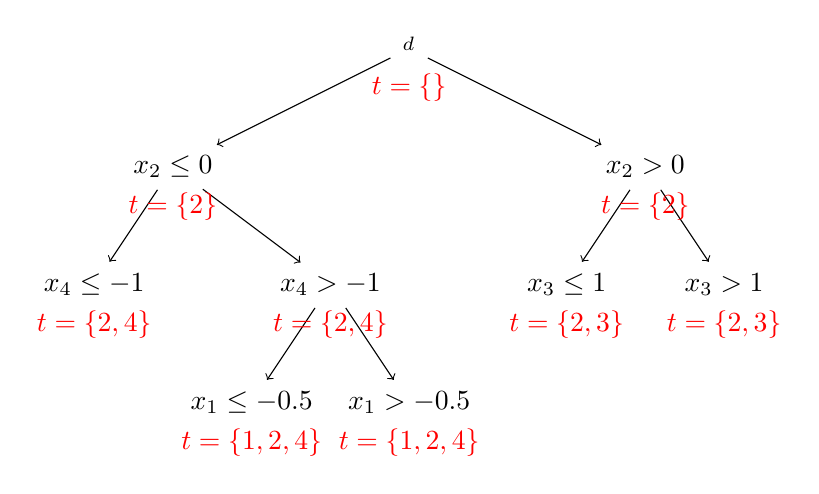
\begin{tikzpicture}[
    node/.style = {scale=1},
    scale = 1
    ]
        
        \node[node] at (0,2)(root){\(\R^d\)};
        
        \node[node] at (3,.5)(right_child){\(x_2 > 0\)};
        \node[node] at (4,-1)(rightright_grandchild){$x_3 > 1$};
        \node[node] at (2,-1)(rightleft_grandchild){\(x_3 \leq 1\)};
        
        \node[node] at (-3,.5)(left_child){\(x_2 \leq 0\)};
        \node[node] at (-4,-1)(leftleft_grandchild){$x_4 \leq -1$};
        \node[node] at (-1,-1)(leftright_grandchild){\(x_4 > -1\)};
        
        \node[node] at (-2,-2.5)(low_child_1){$x_1 \leq -0.5$};
        \node[node] at (-0,-2.5)(low_child_2){$x_1 > -0.5$};

        \draw[->, shorten >= 1pt, shorten <= 1pt] (root) -- (left_child);
        \draw[->, shorten >= 1pt, shorten <= 1pt] (root) -- (right_child);
        \draw[->, shorten >= 1pt, shorten <= 1pt] (left_child) -- (leftleft_grandchild);
        \draw[->, shorten >= 1pt, shorten <= 1pt] (left_child) -- (leftright_grandchild);
        \draw[->, shorten >= 1pt, shorten <= 1pt] (right_child) -- (rightright_grandchild);
        \draw[->, shorten >= 1pt, shorten <= 1pt] (right_child) -- (rightleft_grandchild);
        
        \draw[->, shorten >= 1pt, shorten <= 1pt] (leftright_grandchild) -- (low_child_1);
        \draw[->, shorten >= 1pt, shorten <= 1pt] (leftright_grandchild) -- (low_child_2);

        \only<2>{
        \node[node, color=red] at (0,1.5)(root_type){$t=\{\}$};
        
        \node[node, color=red] at (3,0)(right_child_type){$t=\{2\}$};
        \node[node, color=red] at (4,-1.5)(rightright_grandchild_type){$t=\{2,3\}$};
        \node[node, color=red] at (2,-1.5)(rightleft_grandchild_type){$t=\{2,3\}$};
        
        \node[node, color=red] at (-3,0)(left_child_type){$t=\{2\}$};
        \node[node, color=red] at (-4,-1.5)(leftleft_grandchild_type){$t=\{2,4\}$};
        \node[node, color=red] at (-1,-1.5)(leftright_grandchild_type){$t=\{2,4\}$};
        
        \node[node, color=red] at (-2,-3)(low_child_1_type){$t=\{1,2,4\}$};
        \node[node, color=red] at (0,-3)(low_child_2_type){$t=\{1,2,4\}$};
        
        }

    \end{tikzpicture}
\end{center}
}

\only<2>{
$\Rightarrow$ Degree of interaction in each node is \(|t|\).
}

\only<3>{
[show that one decision tree directly comes with its functional decomposition using indicator functions]\\

Here: $\fh(\xv) = g_0 + g_{2,4}(x_2, x_4) + g_{2,3}(x_2, x_3) + g_{1, 2, 4}(x_1, x_2, x_4)$

\textbf{Problem again: uniqueness} If only reading from decision tree using indicator functions, lower-order effects may be hidden inside higher-order terms? \\

Above example: Decomposition no main effect, but model certainly contains main effect of e.g. $x_2$.\\

\(\Rightarrow\) Solution for that in 
\citebutton{Yang (2024)}{https://arxiv.org/abs/2410.19098} \(\Rightarrow\) Too complicated? Rather explain this in constraint-chapter or in other methods-chapter?
}
    
\end{frame}

\begin{frame}{Example: EBM}

    \begin{itemize}
        \item See before: \textbf{GAMs} have functional decomposition by definition
        \item \textbf{Similar: EBMs} Use the final one- and two-dimensional components visualized in the end
        \item \textit{copy EBM slide here}
        \only<2>{
        \item In general: Model with functional decomposition up to max. order 2 is always ``inherently interpretable''
        \item \textbf{Reason:} Visualization of all components
        } 
    \end{itemize}
    
\end{frame}

\begin{frame}{High-dimensional modl representation (HDMR)}
    [explain link to HDMR?? Or at end of chapter ?]

    same for Sobol-Hoeffding decomposition
\end{frame}








\endlecture
\end{document}
